\documentclass[conference]{IEEEtran}
\IEEEoverridecommandlockouts
% The preceding line is only needed to identify funding in the first footnote. If that is unneeded, please comment it out.
\usepackage{cite}
\usepackage{amsmath,amssymb,amsfonts}
\usepackage{algorithmic}
\usepackage{graphicx}
\usepackage{textcomp}
\usepackage{xcolor}
\def\BibTeX{{\rm B\kern-.05em{\sc i\kern-.025em b}\kern-.08em
    T\kern-.1667em\lower.7ex\hbox{E}\kern-.125emX}}
\usepackage{listings}
\lstset{
  frame=single,
  language=python,
  basicstyle=\small,
}

\makeatletter
\def\lst@makecaption{%
  \def\@captype{table}%
  \@makecaption
}
\makeatother

\begin{document}

\title{CS525 - Team 1 Project 4 Progress Report}

\author{
\IEEEauthorblockN{Alexander Moore}
\IEEEauthorblockA{\textit{Data Science} \\
\textit{Worcester Polytechnic Institute}\\
Worcester, United States \\
ammoore@wpi.edu}

\and

\IEEEauthorblockN{Brian Lewandowski}
\IEEEauthorblockA{\textit{Computer Science} \\
\textit{Worcester Polytechnic Institute}\\
Worcester, United States \\
balewandowski@wpi.edu}

\and

\IEEEauthorblockN{Jannik Haas}
\IEEEauthorblockA{\textit{Data Science} \\
\textit{Worcester Polytechnic Institute}\\
Worcester, United States \\
jbhaas@wpi.edu}

\and

\IEEEauthorblockN{Quincy Hershey}
\IEEEauthorblockA{\textit{Data Science} \\
\textit{Worcester Polytechnic Institute}\\
Worcester, United States \\
qbhershey@wpi.edu}

\and

\IEEEauthorblockN{Scott Tang}
\IEEEauthorblockA{\textit{Data Science} \\
\textit{Worcester Polytechnic Institute}\\
Worcester, United States \\
stang3@wpi.edu}
}

\maketitle

\begin{abstract}
    Understanding which models succeed (and why) at which tasks is a foundational experience in reinforcement learning.
    Following a baseline of techniques and best practices found in the literature this project will show a comparison of multiple reinforcement learning techniques applied in a few common environments.
    In particular, the aim of this project is to implement several Q-learning and policy learning algorithms and compare the results across diverse tasks.
    In addition, the results attained by this work will be analyzed with respect to the expected outcomes of each algorithm on each task.
    This work will serve as an exploration of baseline results for diverse reinforcement learning algorithms, in order to compare and contrast the performance of models on diverse tasks.
    Potential conclusions of this work could include suggestions for appropriate models given the task, heuristic hyperparameters which work for many models, and potential evidence that some models always outperform others, though we expect models to succeed and fail based on the inductive biases their structures assume.
\end{abstract}

\begin{IEEEkeywords}
Q-Learning, Policy Learning, DQN, Policy Gradient, Reinforcement Learning
\end{IEEEkeywords}

\section{Introduction}
Project 3 explored how to construct a Deep Q Network (DQN) by following the classic DQN algorithm outlined originally in \cite{DQNOriginalPaper}.
Building off of this recent experience this project proposes that deep learning techniques applied to the area of policy learning are implemented and compared to the results of DQNs.

In addition, this project proposes to use the \cite{DQNOriginalPaper} breakout screen capture game as a baseline for the environment and games to use for comparison of techniques as it is considered more difficult than the Atari 2600 games contained in the Arcade Learning Environment \cite{Bellemare_2013}. The results on this discrete action-space game will be contrasted to the results of training our set of models on the continuous action space game Box2D BipedalWalker-v2 \footnote{https://gym.openai.com/envs/\#box2d}. Though all of our models can be applied to both discrete and continuous action games, we expect very different results and ideally will find that no one model outperforms all others across both tasks. Time permitting, we can add additional tasks which differ from the previous two games, to refine our sense of why some models would outperform others given the context of the experiment.
Using this environment multiple agents will be trained using policy learning techniques such as vanilla policy gradient, proximal policy optimization (PPO), Monte Carlo policy gradient, with the final cast of models and hyperparameters selected based on compute-time available.

The results of these agents will then be compared to trained Q-learning agents implemented as a DQN, Double DQN, and Dueling DQN; while using the results to assess the strengths and weaknesses of each. By comparing multiple agents across multiple games we will create a case for the superiority or inferiority of some algorithms to others by finding or disproving that there is no one algorithm which consistently outperforms others.

The remainder of this progress report is as follows:
\begin{itemize}
\item Section \ref{background} provides background information regarding the methods planned to be implemented.
\item Section \ref{planned} outlines the specific work done and remaining to be done for this project.
\item Section \ref{deliverables} indicates the expected deliverables to be generated and provided as part of this work.
\item Finally, the proposal concludes in section \ref{conclusion}.
\end{itemize}

\section{Background Information} \label{background}
Our goals may change for implementation. For example, we may focus on a smaller amount of models and instead compare tweaks on these algorithms to demonstrate and quantify the improvement they offer.
\subsection{Deep Q Learning}
Deep Q learning uses a deep neural network to learn coefficients $\omega$ such that the network's value function evaluates $(state, action)$ pairs improving the model's task reward. For some of our environments this will be a convolution over a screen space, and for some we might extract some derived features about the game for the model to use as a state representation.

\subsection{Double Deep Q Learning}
Double deep Q networks address the maximization bias problem from Deep q learning by instead letting two Q functions randomly select the action and update the corresponding Q function. This process inhibits bias and will potentially converge faster or outright outperform DQN on all tasks.

\subsection{Dueling Deep Q Learning}
Dueling DQN separates the Q-learning process into two functions, the sum of the state and state-action estimator models. This approach ideally learns how to relatively value states by accounting for a learned state-value function $V(s)$, as well as an advantage function $A(s,a)$ interpreted as the value of taking action $a$ while in state $s$. For this reason this different approach will be interseting to analyze on tasks where the actions might not always directly affect the environment, for example in breakout where many movements have no direct affect on the game environment.

\subsection{Basic Policy Gradient}
Policy gradient algorithms in general are methods that learn a parameterized policy that can select actions without consulting a value function \cite{ReinforcementLearningBook}.
A value function may be utilized or learned to support learning a given policy, however, it is not involved in the process of choosing an action with these methods \cite{ReinforcementLearningBook}.
The Basic Policy Gradient algorithm treats learning of the policy as an episodic case using a performance measure that equates to the reward obtained following the current policy given a starting state of an episode. 
At its core, the Basic Policy Gradient algorithm takes the gradient of expected rewards for an episode and uses it to update the policy parameters.
This can be summarized by the two equations below,

$$\nabla \bar{R}_{\theta} = \frac{1}{N} \sum \limits_{n=1}^N \sum \limits_{t=1}^{T_n} R(\tau^n) \nabla log\pi_{\theta}(a_{t}^n | s_{t}^n)$$

$$\theta = \theta  + \eta \nabla \bar{R}_{\theta}$$

where N is the number of episodes, T is the steps within an episode, R is the reward for a given episode, $\theta$ are the policy parameters, a is a given action, and s is a given state.

Implemented in pseudocode, this algorithm would be similar to Listing \ref{listing:basicPolicyGradientAlg}.

\begin{lstlisting}[
    float=t,
    caption=\textbf{Basic Policy Gradient} The basic policy gradient algorithm,
    label=listing:basicPolicyGradientAlg,
]

Loop until stopping criteria met:
    for a batch of episodes:
        - Step through episode
        - Store reward gained

    - Determine reward gradient of batch
    - Update policy parameters
\end{lstlisting}

\section{Planned Work} \label{planned}

\subsection{Background Research}
Research is planned to be performed to understand all of the techniques to be exercised during this project.
In addition, the literature will be surveyed to identify any recent developments or improvements related to the methods being employed.
While doing this, we also plan to obtain available benchmarks for techniques such as those found in \cite{DQNOriginalPaper}, \cite{NatureDeepLearning}, and \cite{bhonker2017playing}.
To keep experiments fair to models and reduce compute time, we will find hyperparameter suggestions by model authors where available, but not directly tune one model's hyperparameters for a single game task. Rather, heuristics will be used in their place to attempt to simultaneously generalize models across tasks while keeping experimental design relatively fair.

\subsection{Environment Setup}
This part of the project involves ensuring that all team members have the ability to develop and assess the algorithms under study.
Some of the key areas include ensuring a common (or compatible) software environment is available including the ability to run \cite{nichol2018retro} either locally or on a WPI asset such as the Ace cluster.
In addition, a simple framework or skeleton code should be utilized such that all algorithm implementations are structurally similar.
We plan to take advantage of the provided framework from Project 3 to reduce the amount of work necessary in this area.

\subsection{Algorithm Implementations}
The algorithm implementations involve taking the actual theoretical algorithms and implementing them in Python code using common libraries such as PyTorch and NumPy.
The goal of these implementations is to be true to the algorithms and any notable improvements that have become common in practice.
While deviations and modifications to these algorithms may become necessary for practical reasons, they will be noted in the final report provided, and no modifications would be made which fundamentally alters the bahavior of agents in the games we are testing. The primary goal is to evaluate convergence speed, time to a goal score, and consistency of results across tasks.

\subsection{Results Analysis}
During the analysis of the results each model will be compared using common metrics such reward per episode and the number of episodes necessary for convergence.
In addition, commentary will be provided of any interesting results or findings from the experiments that do not fit into the objective metrics being measured.
We will incorporate our knowledge from researching capabilities of the models as well as our intuitions gained from implementing the algorithms to analyze their performances in both testing and training. After considering case-by-case performances of each model, we can consider the field of agents to determine if there is a subset of 'best' models which consistently outperformed their peers, and maintained that success even across diverse tasks. Ranking quality of models across these tasks can be done with metrics such as training time to achieve a threshold score, max score reached given a limited training time, and consistency of performance across tasks.

\subsection{Work Completed}

Our largest contribution to the final deliverable so far is the development of an agent-game pair running file, in which the researcher inputs arguments into the terminal corresponding to the model and task they would like to dispatch for training. This means all of our model implementations must be written such that they are indifferent to different environment types, state shapes, model attributes, or other quirks arising in agent training. This means that all agents must inherit from a superclass of a general agent framework, and particularities in training (such as the difference between training on state-action-reward tuples, episodes, or tuples of episodes must be addressed in one exectution of the model's unique 'train()' function, which is called in the general 'agent\_runner' executed file.
At the testing time determined by the 'agent\_runner' call, this same process occurs though in a simpler fashion where the generic 'agent.make\_action' refers to a trained policy and state-value function to play the game it was trained on.
The development of this general dispatcher will serve two primary purposes for the remaining work of the project. First, this shared dispatcher file will assure consistent running of each model, where changes can be made to environments and shared parameters without needing to rely on manual changes to many ($num\_tasks*num\_agents$) files. Second, this greatly expedites batch computation when training models on cluster computers, as we can serialize calls for any number of agents, games, and hyperparameters as we see necessary.

We demonstrate some features of this runner structure with the below samples of training-reward snapshots for a DQN model:
\begin{figure}
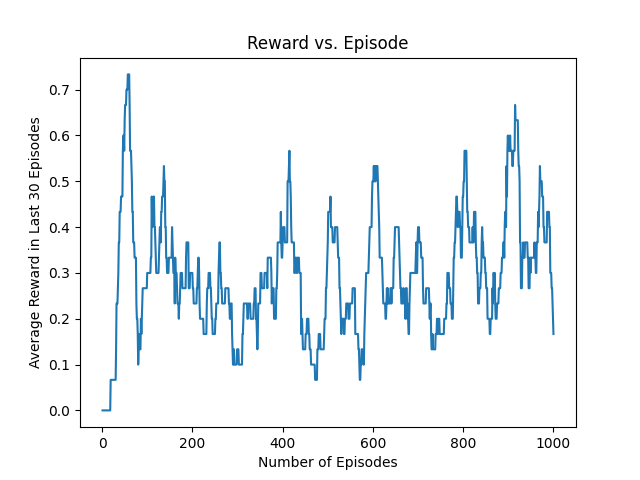
\includegraphics{1000_training_reward_plot.png}
\caption{Training rewards through time, generated by our common runner application}
\end{figure}

\begin{figure}
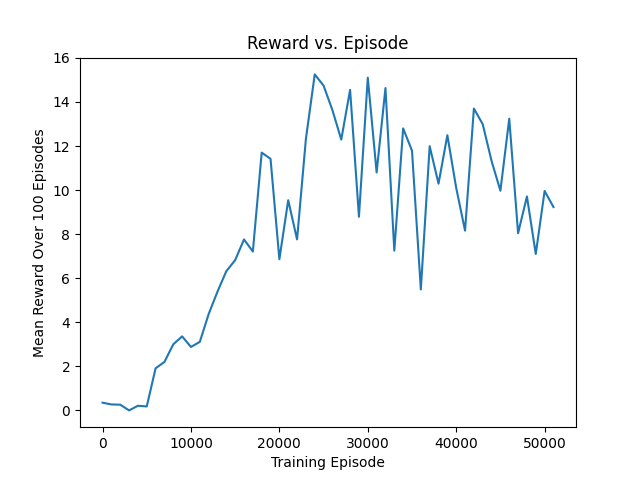
\includegraphics{exp4_test_metrics.png}
\caption{Test metrics of our DQN model, automaticall generated}
\end{figure}

So far, we have draft versions of the following algorithms:
\begin{enumerate}
\item Policy Gradient REINFORCE
\item DQN
\item Double DQN
\item Dueling DQN
\end{enumerate}

The following algorithms are unstarted or in a very early stage:
\begin{enumerate}
\item Policy Gradient PPO
\item Basic Policy Gradient
\end{enumerate}

\subsection{Paper Preparation}
A roughly 10 page paper will be put together to conclude this project and communicate its findings.
This paper will include any background information necessary for the project, a description of algorithms used and considered, implementation methods, results, and analysis.

\subsection{Presentation Preparation}
The work of this project will be summarized in a presentation to be delivered on the poster day for the project.
If any work is found to be an interesting demo it would be displayed during the presentation time. Potential presentation results include:
\begin{itemize}
    \item Expected score in testing after a fixed training time in seconds or iterations for each game
    \item Necessary training time in seconds or iterations to achieve a fixed score for each game
    \item Comparison of learning rates of models for each game
    \item Meta-comparison of games, their action spaces, and relevant challenges and tasks. This will include discussion on the nature of each algorithm as well as our expectations for the performance given the quirks of each task. We will include mathemematical intuition for why some models would struggle or fial to learn in some environments.
\end{itemize}

\section{Tools and Environment}

\subsection{Implementation Language}
This project will be using the Python language of at least version 3.7.
In addition to the standard libraries, it is expected that the following additional libraries will be utilized and standardized across group developement machines:
 
\begin{itemize}
    \item Gym Retro \cite{nichol2018retro}
    \item PyTorch
    \item NumPy
    \item Matplotlib
    \item Pandas
\end{itemize}

In addition, the framework from Project 3 will be utilized as a baseline for implementing the various algorithms being researched. Each algorithm can be fit in this framework to facilitate plug-and-train pipelines for each different model and game.

\subsection{Reinforcement Learning Environment}
This project plans to use an existing reinforcement learning environment while assessing the various algorithm implementations.
In particular, the Retro Learning Environment \cite{nichol2018retro} will be utilized for its large selection of games with high levels of complexity.
We maintain the usage of the Atari Breakout gym environement for multiple reasons. The breakout environment will be familiar to our peers as something they worked extensively with on project 3, and know the implementation tricks as well as the expected rewards of a DQN model, for example. This will contextualize a results plot which shows perhaps that DQN is outperformed by other models, to some comprehensible scale.
In addition, it maintains the same API as the environment used in Project 3 making it close to a drop-in replacement for the existing Project 3 framework with our mentioned extensions to add robustness to model differences, game flexibility, and other algorithm needs.

The initial plan was to focus on the games explored in \cite{bhonker2017playing} as there is a baseline result for several algorithms and a known level of complexity.
Some of the options to be explored include F-Zero, Gradius 3, Mortal Kombat, and Wolfenstein.
We have altered this course to instead use a simple by continuous-space environment provided by the OpenAI Gym. This will lead to stability in comparing the tasks, as the environments are provided by the same source despite the games being very different. In addition a simpler task might lead to more reasonable results, where we know even DQN can have some small success, where we worried that extremely complex games might lead to uninteresting results if some models fail to learn any meaningful parameters during training.
Note that the choice of game is subject to change depending on availability of published results and practical reasons given the time frame for the project.
These games represent diversity in action spaces, reward sparsity, action-memory importance, and state dimensionality.

\subsection{Compute Resources}
The plan for compute resources is to use a combination of local machines as well as the Ace cluster at WPI.
Several team members have access to personal machines with GPUs while other team members have access to the Ace cluster.
These resources combined should provide sufficient computing resources to be successful on this project.
Dispatching batches of jobs to the Turing machine with GPU requirements can also expedite and parallelize long training times.

\section{Work Completed and Ongoing Schedule} \label{deliverables}
This section outlines the schedule for this project on a weekly basis with the main tasks enumerated within the week during which they are expected to complete.
As this is a progres report, at this point we will stick to this schedule to assure that all the main deliverable components are completed on time, and we will expand or retract the scope of the project as necessary to create a motivating and convincing deliverable.

\subsection{Week Ending 11/13}
\begin{enumerate}
    \item Refine Project Idea [Complete]
    \item Develop Project Proposal [Complete]
    \item Submit Project Proposal [Complete]
\end{enumerate}

\subsection{Week Ending 11/20}
\begin{enumerate}
    \item Set up environment infrastructure [Complete]
    \item Determine final list of included algorithms and tasks [Complete]
    \item Research and understand algorithms [Complete]
    \item Begin implementing algorithms [Complete]
\end{enumerate}

\subsection{Week Ending 11/27}
\begin{enumerate}
    \item Continue algorithm implementation [In Progress]
    \item Begin algorithm execution [In Progress]
    \item Refine model hyperparameters as needed
    \item Collect data for analysis
    \item Prepare and deliver project progress report [Complete]
\end{enumerate}

\subsection{Week Ending 12/04}
\begin{enumerate}
    \item Analyze and compare model performance
    \item Begin writing report
    \item Begin working on presentation
\end{enumerate}

\subsection{By Tuesday 12/08}
\begin{enumerate}
    \item Complete report
    \item Complete presentation
    \item Dry run presentation
    \item Submit artifacts
    \item Present findings during poster session
\end{enumerate}

\subsection{Thursday 12/10}
\begin{enumerate}
    \item Present at poster session
\end{enumerate}

\section{Deliverables}

\subsection{Progress Report}
A progress report is planned to be put together and delivered by 11/26 in accordance with the project requirements.
This report is expected to provide a clear picture of progress made on the project to date and the plan for the project over the remainder of the semester.
In addition, any deviations from this proposal will be indicated as necessary in the progress report. At this time any concerns about compute and development time can be brought up to re-evaluate the proposed methods and goals of the project to conclude within the project time.

\subsection{Final Report}
The final report provided as part of this project will include the necessary background information required to understand the methods used.
In addition, our findings on $N*K$ trained models where N is our number of agents and K is our number of games will be included.
The analysis of our findings will include theory on why some models performed better or worse given the game tasks, appropriate model choices for different tasks, and a discussion on our findings of what succeeded and failed for developing diverse models over diverse tasks.
In addition, a description of our methodology will be provided such that others could use our workflow to do the same experiments.

\subsection{Code and Model Artifacts}
All code and artifacts needed to duplicate this project will be provided as part of the deliverables for this project.
In addition, all trained models used in reported performance measures will be saved and provided.

\subsection{Presentation}
The presentation delivered as part of this project will provide an overview of the information covered in the final report.
This includes brief background information and a focus on the comparative results received.
If applicable, any live demos will be rendered and performed during this portion of the project.

\section{Conclusion} \label{conclusion}
This proposal has provided a detailed summary of the planned project including its overall objectives, an outline of the methodology proposed, as well as a detailed schedule.
We welcome any feedback and look forward to exploring this area of reinforcement learning over the next few weeks.

\bibliography{citations.bib}{}
\bibliographystyle{plain}

\vspace{12pt}

\end{document}
